

\documentclass[12pt,a4paper,twoside]{report}
\usepackage{enumitem}
\usepackage{titlesec}  % To make table of contents
\usepackage{amsmath} % Math package for arrays, matrices
\usepackage[utf8]{inputenc} % for single quotes, double quotes
\usepackage{amssymb} % for symbols
\usepackage{array} % for tables
\usepackage{graphicx} % for inserting images
\usepackage[usenames, dvipsnames]{color}
\usepackage{color}
\usepackage[rightcaption]{sidecap}
\usepackage{wrapfig}
\graphicspath{{images/}}
\usepackage{tabularx}
\usepackage[skip=5pt plus1pt, indent=10pt]{parskip}
\usepackage{caption}
\usepackage{subcaption}
\renewcommand\thesubfigure{\roman{subfigure}}
\usepackage{listings}
\lstdefinestyle{mathematica}{
	language=Mathematica,
	basicstyle=\ttfamily,
	columns=fullflexible,
	keepspaces=true,
	commentstyle=\color{gray},
	keywordstyle=\color{blue},
	morekeywords={Plot, Table, Range},
	% Add any additional options or configurations as needed
}
\usepackage{xcolor}
\definecolor{codegreen}{rgb}{0,0.6,0}
\definecolor{codegray}{rgb}{0.5,0.5,0.5}
\definecolor{codepurple}{rgb}{0.58,0,0.82}
\definecolor{backcolour}{rgb}{0.95,0.95,0.92}
\lstdefinestyle{mystyle}{
	backgroundcolor=\color{backcolour},   
	basicstyle=\ttfamily\footnotesize,
	breakatwhitespace=false,         
	breaklines=true,                 
	captionpos=b,                    
	keepspaces=true,                 
	numbers=left,                    
	numbersep=5pt,                  
	showspaces=false,                
	showstringspaces=false,
	showtabs=false,                  
	tabsize=2
} 
\lstset{
	language=Python,
	basicstyle=\ttfamily\small,
	keywordstyle=\color{blue},
	commentstyle=\color{green!60!black},
	stringstyle=\color{orange},
	showstringspaces=false,
	tabsize=4,
	frame=single,
	numbers=left,
	numberstyle=\tiny,
	numbersep=5pt,
	breaklines=true,
}
\lstset{style=mystyle}
\usepackage{fancybox}
\usepackage{fancyhdr}
\pagestyle{fancy}
\fancyhf{}
\fancyhead[LE,RO]{Shivaji College}
\fancyhead[RE,LO]{MRP/2021/0004}
\fancyfoot[CE,CO]{\leftmark} % chapter name center
\fancyfoot[LE,RO]{\thepage}  % page no. left n right
\renewcommand{\headrulewidth}{1pt}
\renewcommand{\footrulewidth}{1pt} 
\usepackage{tgbonum}
\pagenumbering{arabic}
\usepackage{imakeidx}
\makeindex[columns=3, title=Index, intoc]
\titlespacing\chapter{0pt}{12pt plus 2pt minus 2pt}{12pt plus 2pt minus 2pt}
\titlespacing\section{0pt}{14pt plus 4pt minus 2pt}{14pt plus 2pt minus 2pt}
\titlespacing\subsection{0pt}{12pt plus 4pt minus 2pt}{12pt plus 2pt minus 2pt}
\titlespacing\subsubsection{0pt}{12pt plus 4pt minus 2pt}{12pt plus 2pt minus 2pt}
\usepackage[spaces,hyphens]{url}
\usepackage{ragged2e}


\begin{document} %Document Is Initiated
\begin{titlepage}
		\begin{figure}[htb]
			\centering
			\begin{subfigure}[h]{0.3\textwidth}
				\centering
				
\includegraphics[width=0.8\textwidth]{ias.png}
			\end{subfigure}%
			\begin{subfigure}[h]{0.3\textwidth}
				\centering
				
\includegraphics[width=0.8\textwidth]{insa.png}
			\end{subfigure}%
			\begin{subfigure}[h]{0.3\textwidth}
				\centering
				
\includegraphics[width=0.8\textwidth]{nasi.png}
			\end{subfigure}%
		\end{figure}
		
	   \begin{center} 
	   	
	   	
		\vspace{1cm} %Space   
		\Huge
		\textbf{Mapping the Nature of Light Reflections by a Reflective Curve in Cartesian Plane}
		
		\begin{figure}[h]
			\centering
			
\includegraphics[width=0.7\textwidth]{iisc.png}
		\end{figure}%
		
		\normalsize
		\textbf{Applicant Number:} \textit{MATS142}
		
		\vspace{0.5cm} %Space
		
		\textbf{Summer Research Fellow}:\\ Raghav Anand Nath\textit{~(University Of Delhi, Delhi)} \vspace{0.3cm}\\ \textbf{Guide} : \\  Dr. Ramsharan Rangarajan \textit{~(Indian Institute of Science, Bengaluru)}
		
%		\vspace{0.8cm} %Space
%		\includegraphics[width=0.25\textwidth]{}
%		\includegraphics[width=0.4\textwidth]{}   
		
		\vspace{1.2cm} %Space
		\textbf{Summer Research Fellowship Programme 2023}\\	         
	\end{center}
\end{titlepage}

\begin{abstract}
	\vspace{1cm}
	The present study explores the behaviour of successive light reflections when encountering an unknown reflective curve and a known reflecting line. We aim to gain insights into the characteristics of such reflective curves through the analysis of the light reflections. \\
	
	The investigation employs three distinct approaches: 
	\begin{enumerate}
	\item Cata-caustics/Differential Geometry Approach
	\item	Combinatorial Elimination
	\item	Reinforcement Learning For Optimal Paths \\
	\end{enumerate} 

	
	Through a comprehensive analysis of the methodologies, we can uncover more information about the nature while simultaneously minimizing the error in its subsequent interpolation of the reflective curve.
	
	
\end{abstract}
\newpage
\pagestyle{empty}

\centering
\vspace{4cm}
\textbf{Acknowledgement}\\ \vspace{1.4cm}
\justifying

I am sincerely thankful to Dr. Ramsharan Rangarajan for his invaluable guidance and unwavering support throughout this project. I am also grateful to the Mechanics and Computation Lab at IISc Bangalore for giving me the opportunity to work on this project.

I deeply appreciate Mr. Chiraprabha Bhattacharyya and all the lab members for their constant support and guidance, helping me at every step of this journey. Their encouragement and insights have been very valuable to me. 

I am also thankful to my professor, Dr. Neetu Rani, and my friends at Shivaji College, DU, for understanding my situation and assisting with college responsibilities while I was away. 

I want to acknowledge the collective support of all these individuals and institutions, as this report would not have been possible without them. I am truly grateful for their contributions to this project. \\

\begin{flushright}
	
	 \textit{Raghav Anand Nath}
\end{flushright}
\tableofcontents{}
\listoffigures



\chapter*{Introduction}
\addcontentsline{toc}{chapter}{Introduction}
\section{Problem Statement}
In a Cartesian plane, consider two distinct sets of points denoted as $A$ and $B$. $A$ exclusively consists of points located along the $x-axis$, serving as a reflective plane mirror. Conversely, $B$ comprises points positioned along an unknown, arbitrary reflective curve represented by $f(x)$. These points represent the locations where a ray of light, originating from the origin and striking point $P$ (which belongs to $B$), undergoes successive reflections. The subsequent reflections occur alternately between the X-axis and the curve in pairs. Given this configuration, determine the nature of the reflective curve $f(x)$.

\begin{figure}[h]
	\centering
	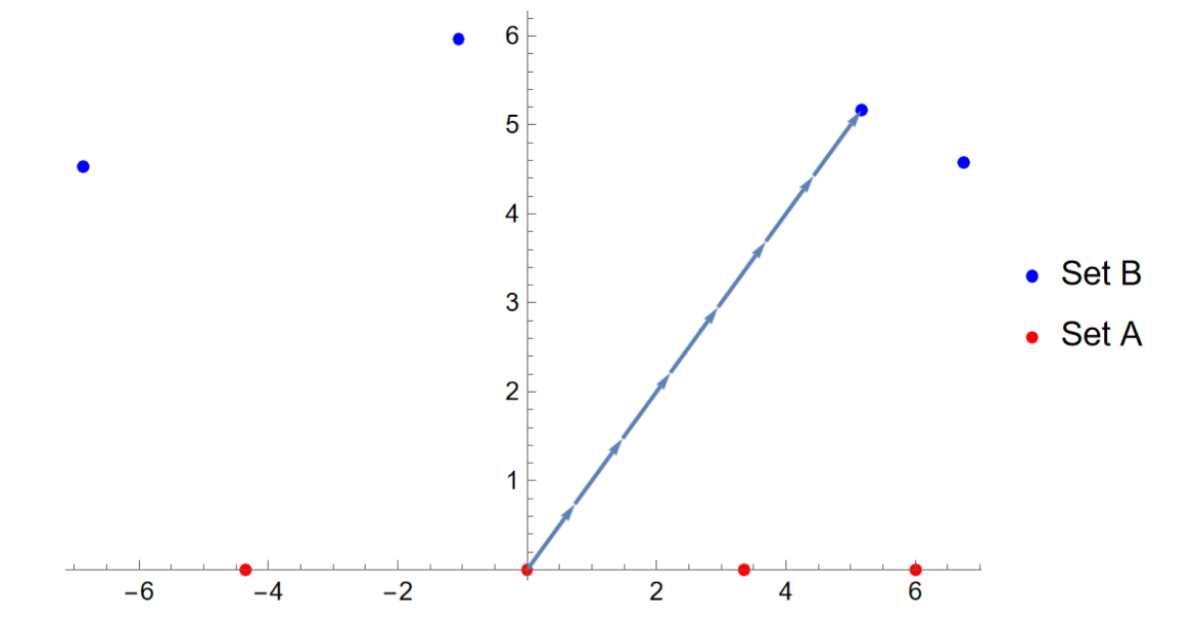
\includegraphics[width=1\textwidth]{pic1.png}
	\caption{~8 Incident Point Configuration}
\end{figure}
\begin{figure}[h]
	\centering
	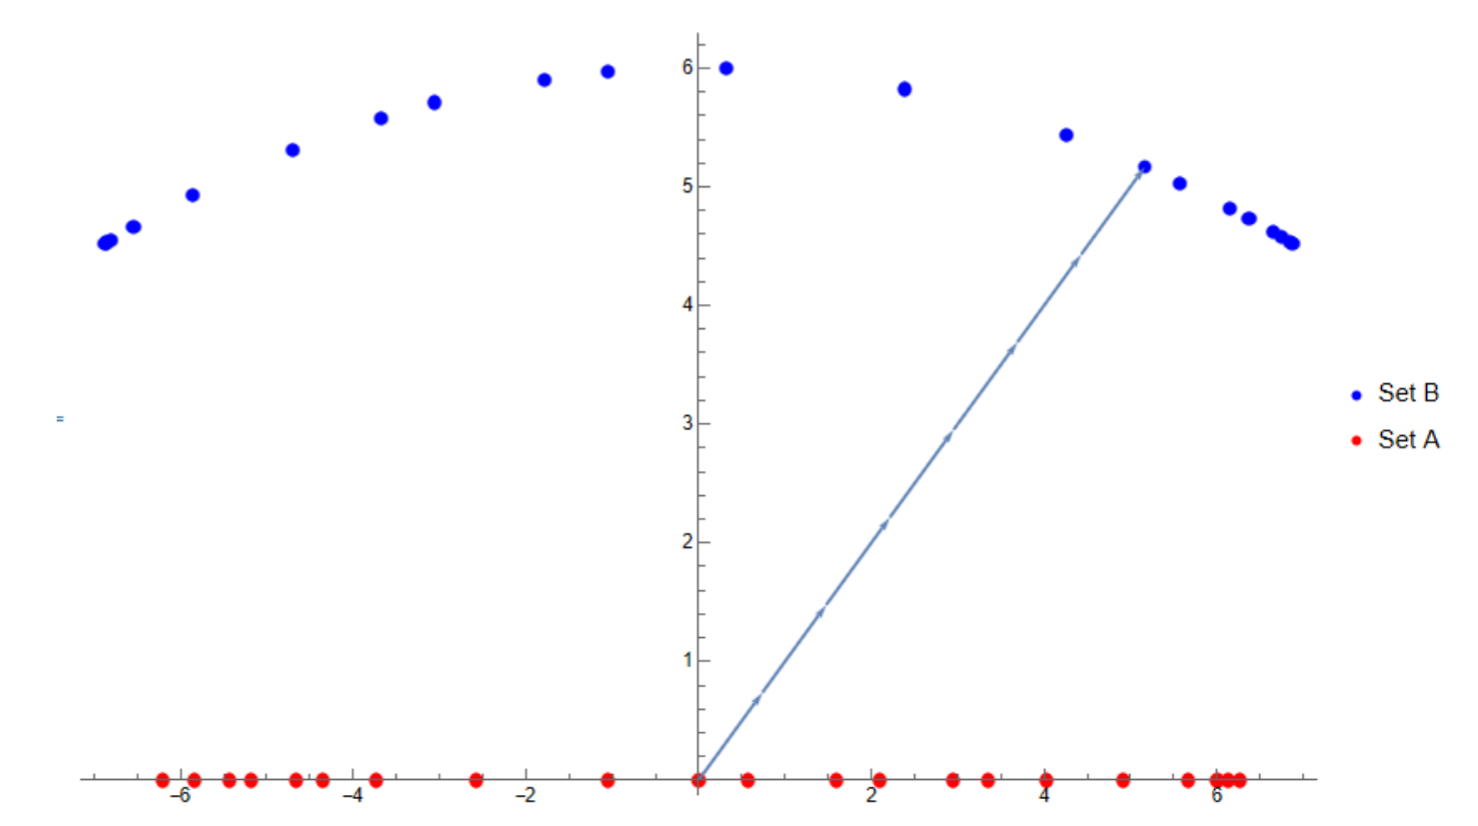
\includegraphics[width=1\textwidth]{pic2.png}

\caption{~42 Incident Point Configuration}
\end{figure}

\section{Significance}
Instead of opting for a straightforward curve fitting approach, which may not yield accurate results, we pursued a more comprehensive solution by tracing the path of light. This allowed us to gather additional information about the derivatives i.e normals and tangents at various points along the curve, enhancing the accuracy of the interpolation. In conclusion, our aim was to obtain crucial information solely from the available incident points of light to achieve a more precise curve interpolation.

\chapter{Methodology}
\section{Caustics and Orthotomics}
\justifying

\textbf{Caustics:}  The curve which is the envelope of reflected (catacaustic) or refracted (diacaustic) rays of a given curve for a light source at a given point (known as the radiant point). \cite{caustic}

\begin{figure}[h]
\begin{subfigure}[h]{0.4\textwidth}
	\centering
	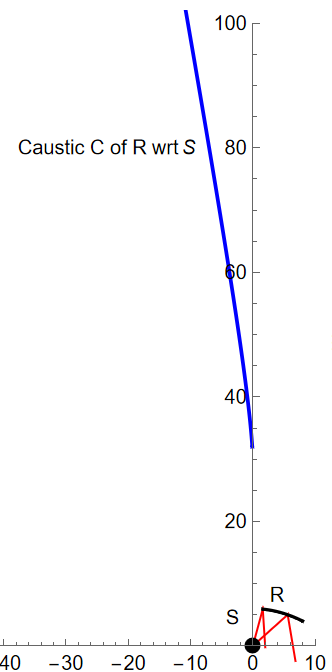
\includegraphics[height=250pt]{caustic.png}
	\caption{~Caustic Curve}
\end{subfigure}
\begin{subfigure}[h]{0.5\textwidth}
	\centering
	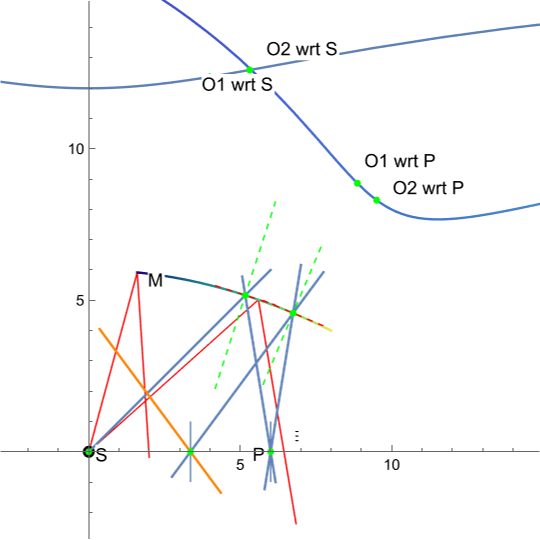
\includegraphics[height=250pt]{ortho.png}
	\caption{~Orthotomic Curve}
\end{subfigure}
\caption{~Caustics and Orthotomics}

\end{figure}

\textbf{Orthotomics:}  Given a source $S$ and a curve $R$, pick a point on $R$ and find its tangent $T$. Then the locus of reflections of S about tangents $T$ is the orthotomic curve (also known as the secondary caustic). \cite{ortho} 

\textit{Note - In the case of caustics, we considered the set of points on the curve as point tangents, giving us the information about the coordinates and tangent information of the curve at the respective coordinates} \\

In our study, we utilized orthotomics to establish a connection between the curve and the caustics formed by the light reflections. However, despite our efforts, we could not find a one-to-one mapping between the caustics and orthotomics with the curve while maintaining a lower degree of derivative value for preserving more information.

In the existing literature, researchers have often assumed continuous curves for both orthotomics and caustics \cite{giblin}\cite{russian}, enabling them to establish equations for the unknown reflecting curve. However, in our case, the values were discrete coordinates without continuity, making it challenging to derive a comprehensive function for the unknown reflective curve. As a result, we could only achieve a two-point mapping of the caustic and orthotomic with respect to the incident point on the curve and the light source. Unfortunately, this mapping did not provide much utility in our analysis, and ultimately, its accuracy was comparable to directly fitting the curve through the incident points.

In conclusion, due to the limitations mentioned above, the caustic and orthotomic approach did not yield the desired results. Consequently, we pursued alternative methods for our investigation.

\newpage
\section{Combinatorial Elimination}

\subsection{Theory}

The configuration of incident points presents a multitude of paths between two points, with $N$ x $M$ possible permutations, where $N$ and $M$ represent the number of points on the $x-axis$ and the curve, respectively. These paths arise from the alternating sequence of light traveling between the $x-axis$ and the $curve$. Restricts such as no backtracing of light, known origin, strict alternate pairs may reduce the combinations further.

To find the correct path, a combinatorial approach is adopted, where various permutations are explored and subsequently filtered based on certain constraints. In this study, the constraint of the $x-axis$ acting as a plane mirror is employed. By utilizing the normal and tangent information at the points of incidence on the $x-axis$, we can deduce crucial information about the reflected ray of light, including the reflection angle and the equation of the reflected ray. This approach proves essential in determining the accurate path of the light ray based solely on its incidence on the $x-axis$.

By considering the equations of reflected rays, we filter out paths that fail to satisfy any incident points on the curve. It is essential to eliminate such paths, as a ray of light reflected by the $x-axis$ must intersect with a point on the curve. Subsequently, we reach another point on the curve, and the process of permutation, filtering, and path evaluation continues iteratively. Since we lack tangent and normal information for the incident points on the $curve$, we perform permutations for these points, filter the paths, and repeat the process until we reach the end of the path.



\begin{figure}[h]
	\centering
	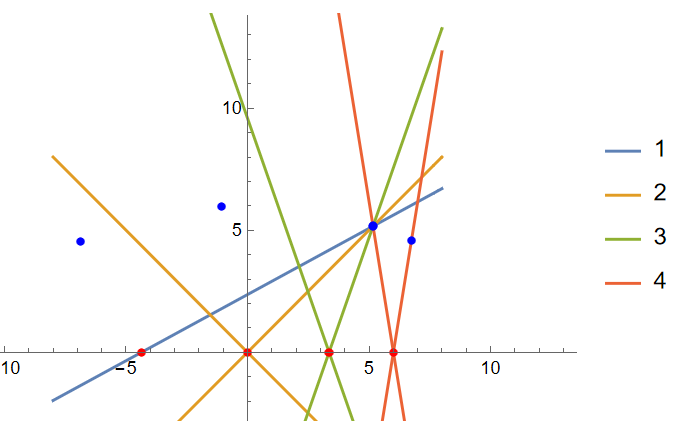
\includegraphics[height = 0.5\textwidth]{combth.png}
	
	\caption{~Reflected Equations Filtering}
\end{figure}

In summary, our combinatorial approach utilizes the constraints of the plane mirror and the available information on normal and tangent vectors to identify the valid path of light reflections between the $x-axis$ and the $curve$ points. This iterative process ensures that the selected paths satisfy the conditions of reflection at the $x-axis$ and intersection with points on the $curve$, leading us to the desired outcome.

The illustration reveals that the reflected rays labeled as $2$ and $3$ and fail to align with any incident point following reflection from the plane mirror ($x-axis$). Consequently, these rays are eliminated, and equation $4$ is identified as the valid path of light reflection.

\subsection{Algorithm}

\textit{In the computational simulations conducted using Wolfram Mathematica Ver 12.3, the following steps were followed:}\\

\textbf{Step 1:} The initial input consisted of information about the incident points. These points were subsequently categorized into two sets based on their y-coordinate values: the points lying on the X-axis (representing the plane mirror) and the incident points on the unknown reflective curve. \\

\begin{lstlisting}[style=mathematica]
For[xaxispts = {}; i=0, i<Length[intersecpts], i++; If[intersecpts[[i, 2]]==0, AppendTo[xaxispts, intersecpts[[i]]]]]
curvepts = Sort[DeleteCases[intersecpts, Alternatives @@ xaxispts]];
xaxispts = Sort[xaxispts];
Print["curvepts = ", curvepts]
Print["xaxispts = ", xaxispts]
intersecplot2 = ListPlot[{#} & /@ intersecpts, PlotRange->Full,PlotStyle->{Blue, Red, Blue, Red, Blue, Red, Blue, Red}]
\end{lstlisting}



\textbf{Step 2:} Without considering the initial knowledge of the first incident of the ray of light, all possible 3-point permutation pairs were formed to represent the various paths the light could take before encountering the constraint imposed by the first plane mirror. 

\begin{lstlisting}[style=mathematica]
	pttuplefunc[domainls_, codomainls_]:=
	Module[{tupleset={}},
	For[i=0, i<Length[domainls], i++;
	For[j=0, j<Length[codomainls], j++;
	For[k=0, k<Length[domainls], k++;
	tupleset = AppendTo[tupleset, {domainls[[i]],codomainls[[j]], domainls[[k]]}];
	]]];
	Return[tupleset, Module]];
\end{lstlisting}
There are are a total of 64, three Point Paths available in an 8 incident configuration.

\textbf{Step 3:} The paths were then systematically eliminated based on the constraint, continuing this process iteratively until a unique end path was obtained.

\begin{lstlisting}[style=mathematica]
(*Function to check for the curve points lying on the reflected ray *)
reflecdrop[domainls_] := 
Module[{tupleset = {}}, 
For[i=0, i<Length[domainls], i++;
For[(eqn = y == -(Last[List @@ Reduce[y - InterpolatingPolynomial[{Part[domainls[[i]],-2], Part[domainls[[i]],-1]},x]==0,y]]));
j=0, j<Length[curvepts], j++;
If[(eqn /. {x->curvepts[[j,1]], y->curvepts[[j,2]]})== True, 
tupleset = AppendTo[tupleset,Join[domainls[[i]], {curvepts[[j]]}]]]]];
Return[tupleset, Module]];
\end{lstlisting}

\textbf{Unified function for easier processing \\}
\begin{lstlisting}[style=mathematica]
	merge[list_]:=Module[{a= reflecdrop[list]}, Return[path2func[a], Module]];
	function[list_]:= Module[{a, new={}},
	If[EvenQ[Length[intersecpts]]==True, a = reflecdrop[Nest[merge, list, (Length[intersecpts]-4)/2]],a = Nest[merge, list, (Length[intersecpts]-3)/2]];
	For[i=0, i<Length[a], i++;
	If[CountDistinct[a[[i]]]==Length[intersecpts], new = AppendTo[new, a[[i]]]]];
	Return[new, Module]];
	ListLinePlot[finalpath[[1]], PlotMarkers->{Automatic, 8}, Axes->True, AxesOrigin->{0,0}, MeshFunctions -> {#2 &}, Mesh -> 6, MeshStyle -> Opacity[0], 
	MeshShading -> {Arrowheads[Small]}, DataRange -> {0, 4 Pi}] /. Line -> Arrow 
\end{lstlisting}

\subsection{Path Plots}
\begin{figure}[h]
	\begin{subfigure}[h]{0.5\textwidth}
		\centering
		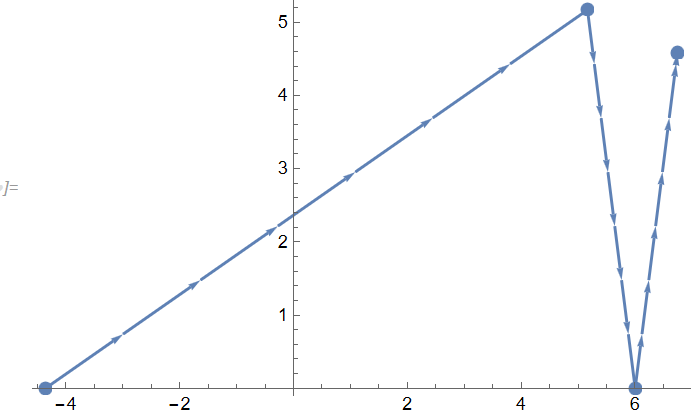
\includegraphics[width=\textwidth]{4pointpath.png}
		\caption{~A 4 Point Path}
	\end{subfigure}
	\begin{subfigure}[h]{0.5\textwidth}
		\centering
		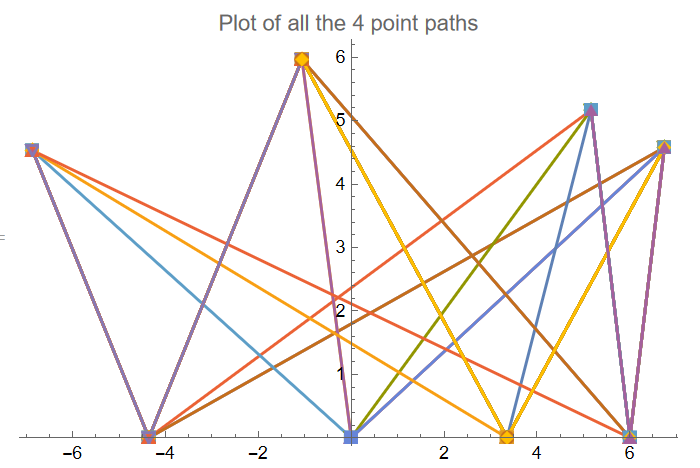
\includegraphics[width=0.9\textwidth]{4pointall.png}
		\caption{~All 4 Point Paths}
	\end{subfigure}
	\caption{~4 Point Paths}
	
\end{figure}

\begin{figure}[h]
	\begin{subfigure}[h]{0.5\textwidth}
		\centering
		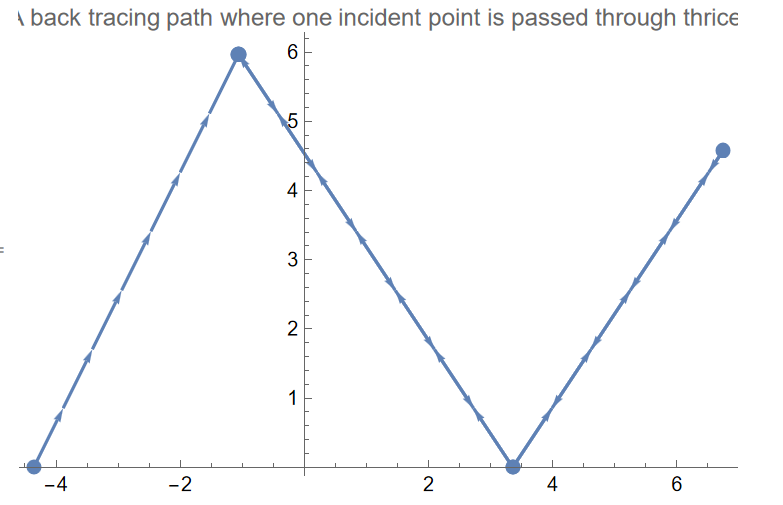
\includegraphics[width=\textwidth]{5pointpath.png}
		\caption{~Backtracing Case Path}
	\end{subfigure}
	\begin{subfigure}[h]{0.5\textwidth}
		\centering
		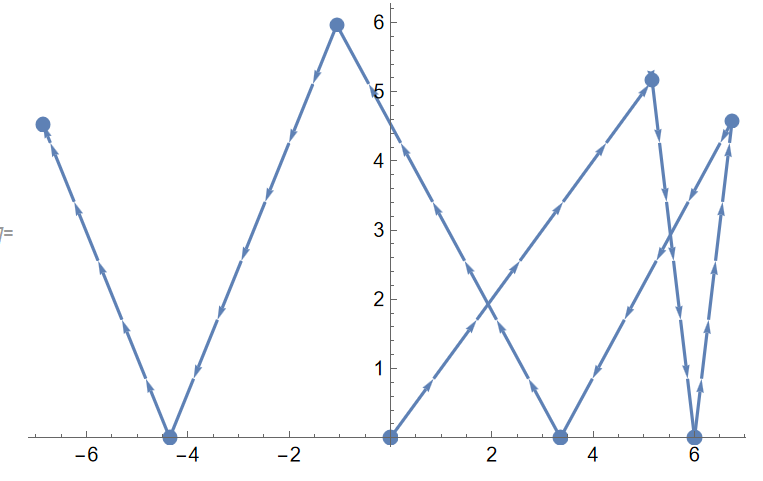
\includegraphics[width=1\textwidth]{finalpath.png}
		\caption{~Final Path}
	\end{subfigure}
	\caption{~5 Point Path and Final Path}
	
\end{figure}

\subsection{Limitations}
The conditions under which the described approach is not applicable are as follows: when the incident points alternate between the curve and the plane mirror, with no consecutive occurrences of light incidents on either the curve or the X-axis, and when the number of iterations is limited during back tracing.

On the other hand, the method is applicable in scenarios where there is no information available about the source point of light, allowing for multiple incidents on the same point, and accommodating the possibility of light retracing its path back.

\subsection{Scope For Improvement}
Leveraging the knowledge of the normals at the points of incidence on the plane mirror, we initiate a procedure involving the generation of permutations. This process entails selecting two points from curve and one point from x-axis, and subsequently filtering out permutations where the slopes of the interpolated line connecting the two sets of points adhere to the reflection transformation. By doing so, we can construct an undirected graph network consisting of valid paths that can be utilized within our proposed methodology

\begin{figure}[h]
	\centering
	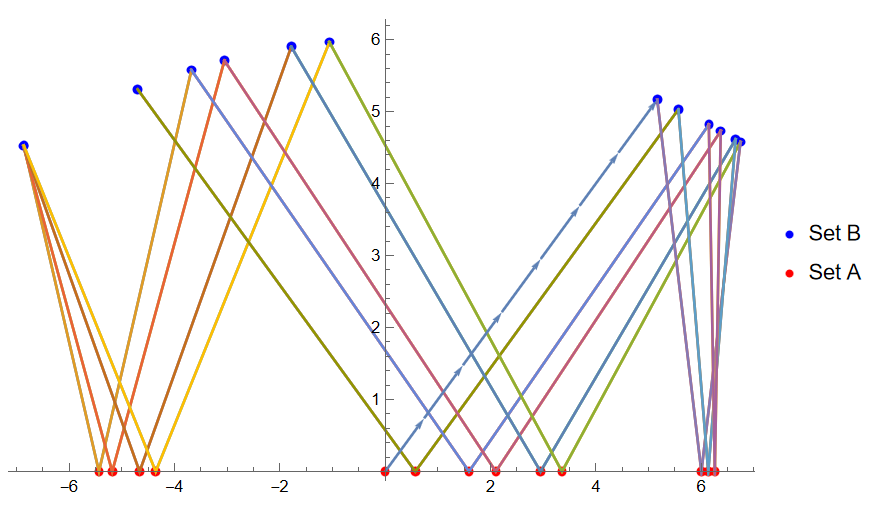
\includegraphics[width=0.8\textwidth]{pic5}
	\caption{~Undirected legal paths}
\end{figure}

\newpage
\section{Reinforcement Learning For Optimal Path}
\subsection{Theory}

The main idea behind this approach is to observe how light rays reflect off a curved surface. When light hits a curved surface, it follows the law of reflection, where the angle at which it strikes the surface is equal to the angle at which it bounces off. The goal is to optimize the angles of incidence and reflection to find the most accurate reflection path. \\

Method:

\begin{itemize}


\item Environment Setup: The Cartesian plane serves as the environment where the reflective curve and light source are situated. The reflective curve is represented as a set of points, and the light source emits rays in various directions.

\item Reinforcement Learning (Q-learning): Q-learning is employed as the learning algorithm for the model. The Q-value represents the expected reward of taking an action (choosing a direction for the light ray) from a given state (a point on the reflective curve). The model learns from the rewards obtained during the simulation to improve the reflection angles.

\item Optimization Objective: The objective of the model is to maximize the sum of the negative of absolute differences between the angles of incidence and reflection for a set of three points (one from the reflective curve and two from the x-axis). This allows the model to optimize the reflection angles and find the most accurate reflection path.

\item Analysis and Visualization: The results of the simulations are analyzed to gain insights into the nature of light reflections by the reflective curve. Visualization techniques are employed to provide a clear representation of the optimized reflection paths and their comparison to the incident paths.\\
\end{itemize}

In conclusion, we aim to understand light reflections off a reflective curve in a Cartesian plane. By using Q-learning and optimizing the reflection angles, we can observe how the curved surface influences the path of light rays.

\subsection{Algorithm}

\begin{figure}
	\centering
	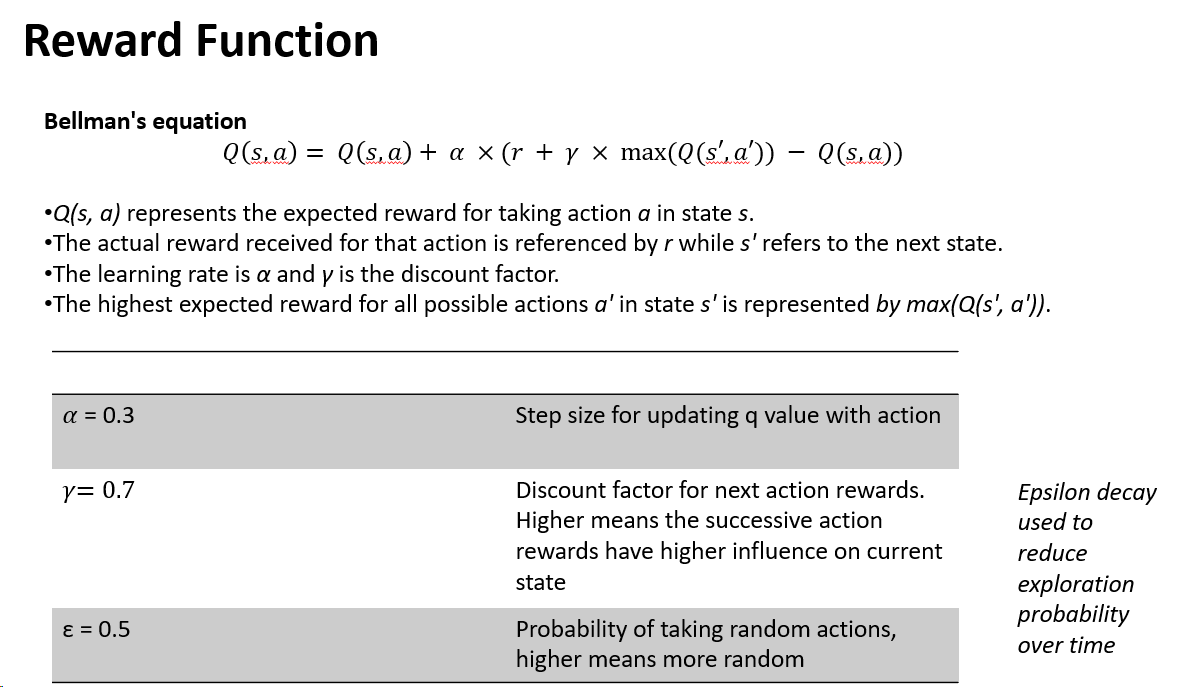
\includegraphics[width=1\linewidth]{rewardfunc}
	\caption{~Bellman's Equation and Hyper-parameters}
	\label{fig:rewardfunc}
\end{figure}

\subsubsection{Simulation of Environment}
\textit{The computational simulations of the enivorment were conducted using Wolfram Mathematica Ver 12.3, subsequently they were exported to the local jupyter notebook,}\\

\begin{lstlisting}[style=mathematica]
(* Function to calculate the reflection angle at a given incident point on the curve *)
curverefangle[incipt_, prevrefangle_] := 
Reduce[(prevrefangle - (-1/(D[curvecarteqn, x] /. {x -> incipt[[1]]})))/(1 + prevrefangle*(-1/(D[curvecarteqn, x] /. {x -> incipt[[1]]})))
== ((-1/(D[curvecarteqn, x] /. {x -> incipt[[1]]})) - m)/(1 + (-1/(D[curvecarteqn, x] /. {x -> incipt[[1]]}))*m), m];

(* Function to calculate the equation of the reflected ray corresponding to a given incident point and reflection angle *)
curverefeqn[incipt_, refangle_] := Reduce[y - (curvecarteqn /. {x -> incipt[[1]]}) == Last[List @@ refangle]*(x - ({x} /. {x -> incipt[[1]]})[[1]]), y];

(* Function to find the point of incidence on the X-axis corresponding to the given reflected ray *)
plincipt[refeqn_] := {x /. Solve[refeqn /. y -> 0][[1]][[1]], 0};

(* Function to calculate the equation of the reflected ray corresponding to the given incident point and reflection angle *)
plrefeqn[incipt_, angle_] := Last[List @@ Reduce[y - 0 == -Last[List @@ angle]*(x - incipt[[1]]), y]];

(* Function to find the point of incidence on the curve corresponding to the given reflected ray *)
curveinci[plrefeqn_] := Module[{b},
For[z = N[Solve[plrefeqn == curvecarteqn, x]]; i = 0, i < Length[a], i++;
If[(x /. z[[i]]) > -10 && (x /. z[[i]]) < 10, b = {x /. z[[i]], curvecarteqn /. z[[i]]}]
];
b
]

(* Initialize empty lists to store equations and points *)
eqnlist = {};
ptlist = {{0, 0}, {5.166010488516726`, 5.166010488516724`}};

(* Function to merge incidents, calculate reflection angles, and find new points *)
mergefunction[list_] := Module[{},
(* Calculate reflection angle *)
a = curverefangle[list[[1]], list[[2]]];
(* Calculate equation of reflected ray *)
b = curverefeqn[list[[1]], a];
(* Find point of incidence on X-axis *)
c = plincipt[curverefeqn[list[[1]], a]];
(* Calculate equation of reflected ray for X-axis incidence point *)
d = plrefeqn[c, a];
(* Find point of incidence on the curve *)
e = curveinci[d];

(* Append equations and points to respective lists *)
eqnlist = AppendTo[eqnlist, {Last[List @@ b], d}];
ptlist = AppendTo[ptlist, c];
ptlist = AppendTo[ptlist, e];

(* Return the new reflected ray *)
{e, -Last[List @@ a]}
]

(* Iteratively trace reflections up to 6 times *)
Nest[mergefunction, {{5.166010488516726`, 5.166010488516724`}, 1}, 6]

(* Display the resulting equations and points *)
eqnlist;
ptlist;

\end{lstlisting}

The provided code is an algorithm to trace the path of light reflections on an unknown reflective curve in the Cartesian plane. It involves calculating reflection angles, finding the equations of reflected rays, and determining points of incidence on the curve and X-axis.

It involves the following concepts - 
\begin{itemize}
\item Reflection Angle Calculation:
The code calculates the angle at which light reflects when it hits a point on the curve. It uses the slope of the curve at that point to find the reflection angle.

\item Equation of Reflected Ray:
The code calculates the equation of the path the light follows after reflecting from the curve. It uses the curve's equation and the reflection angle to find this path.

\item Finding Incident Points:
The code determines the points where the light hits the X-axis and the curve after each reflection. It finds the intersection points of the reflected rays with the X-axis and the curve.

\item Tracing Reflections:
The code repeats the process of finding reflection angles, equations of reflected rays, and incident points for multiple reflections. This allows it to trace the path of light as it reflects off the curve multiple times.
\end{itemize}

\subsubsection{Reinforcement Learning}
\begin{lstlisting}
# Base Data Science snippet
import pandas as pd
import numpy as np
import matplotlib.pyplot as plt
import os
import time
from tqdm import tqdm_notebook
from scipy.spatial.distance import cdist
import imageio
from matplotlib.patches import Rectangle
from matplotlib.collections import PatchCollection

plt.style.use("seaborn-dark")

import sys
sys.path.append("../")
from rl.agents.q_agent import QAgent


\end{lstlisting}

The snippet includes important libraries such as pandas, numpy, and matplotlib, which are essential for handling data, performing numerical operations, and creating plots. Additionally, I imported modules for specific tasks like image processing and progress monitoring.

To enhance the visual aesthetics of the plots, I applied the "seaborn-dark" style to the visualizations. This style provides a clean and appealing appearance to the plots generated throughout the project.

To facilitate reinforcement learning tasks, I imported a custom module called "QAgent," which will be employed in subsequent stages for implementing reinforcement learning algorithms.

To kickstart the data analysis, I loaded the initial dataset from the file 'test.csv' using the 'np.loadtxt' function from numpy. This dataset contains coordinate points representing the Cartesian plane, with two columns representing the x and y coordinates, respectively.

\begin{lstlisting}
xy = np.loadtxt('test3.csv', delimiter=",")

#Separate x axis and curve pts 
def ptseparator(array):
xaxis = list(list())
curve = list(list())
for i in array:
if i[1]==0:
xaxis.append(i)
else:
curve.append(i)
return xaxis, curve  

xaxis, curve = np.array(ptseparator(xy))
print("xaxis array = \n", xaxis)
print("curve array = \n", curve)
\end{lstlisting}

The code loads coordinate points representing the Cartesian plane from the file 'test3.csv'. It then separates the points into two sets: one for the x-axis and the other for the unknown reflective curve based on their y-coordinate values. The resulting sets are displayed for further analysis in the project.

\begin{lstlisting}
import matplotlib.pyplot as plt
import numpy as np

class Environment(object):
def __init__(self, curve, xaxis, method="angle_difference", **kwargs):
# Initialization
print(f"Initialized Delivery Environment with {len(curve) + len(xaxis)} random stops")
print(f"Target metric for optimization is {method}")

# Initializaiton 
self.n_stops = len(curve)
self.curve = curve
self.xaxis = xaxis
self.action_space = self.n_stops
self.observation_space = self.n_stops
self.stops = [0]  # Initialize the list of stops with the starting point (index 0)
self.method = method

# Generate Stops 
self._generate_stops()
self._generate_q_values()
self.render()

def _generate_stops(self):
# Extract x and y coordinates from the 'curve' and 'xaxis' arrays
self.xc = self.curve[:, 0]
self.yc = self.curve[:, 1]
self.xp = self.xaxis[:, 0]
self.yp = self.xaxis[:, 1]

def _generate_q_values(self):
# Calculate the Q-values for all possible combinations of stops and destinations
curve = np.array(self.curve)
xaxis = np.array(self.xaxis)
mat = np.zeros((len(curve), len(curve), len(xaxis)))

for z in range(len(xaxis)):
slope1 = (curve[:, 0] - xaxis[z][0]) / curve[:, 1]
slope2 = (curve[:, 0] - xaxis[z][0]) / curve[:, 1]
diff = -np.abs(slope1[:, None] + slope2)
mat[:, :, z] = diff

self.q_stops = mat

def render(self, return_img=False):
# Visualize the environment with matplotlib
fig = plt.figure(figsize=(7, 7))
ax = fig.add_subplot(111)
ax.set_title("Paths")

# Show stops
ax.scatter(self.xc, self.yc, c="red", s=50)  # Red points represent stops in the 'curve'
ax.scatter(self.xp, self.yp, c="blue", s=50)  # Blue points represent stops in the 'xaxis'

# Show Start
xy = [0., 0.]
xytext = xy[0] + 0.1, xy[1] - 0.05
ax.annotate("START", xy=xy, xytext=xytext, weight="bold")

# Show Itinerary
if len(self.stops) > 1:
self.xarr = [self.xp[0]]
self.yarr = [self.yp[0]]

for i in range(len(self.stops)):
if i % 2 == 0:
self.xarr.append(self.xc[self.stops[i]])
self.yarr.append(self.yc[self.stops[i]])
else:
self.xarr.append(self.xp[self.stops[i]])
self.yarr.append(self.yp[self.stops[i]])

ax.plot(self.xarr, self.yarr, c="blue", linewidth=1, linestyle="--")

# Annotate END
xy = self._get_xy(initial=False)
xytext = xy[0] + 0.1, xy[1] - 0.05
ax.annotate("END", xy=xy, xytext=xytext, weight="bold")

plt.xticks([])
plt.yticks([])

if return_img:
# From https://ndres.me/post/matplotlib-animated-gifs-easily/
fig.canvas.draw_idle()
image = np.frombuffer(fig.canvas.tostring_rgb(), dtype='uint8')
image = image.reshape(fig.canvas.get_width_height()[::-1] + (3,))
plt.close()
return image
else:
plt.show()


def reset(self):
# Reset the environment to the initial state (with only the starting point)
self.stops = [0]
return self.stops[-1]

def _get_state(self):
# Get the current state (last stop)
return self.stops[-1]

def _get_xy(self, initial=False):
# Get the x, y coordinates of the current state (last stop) or the initial state (first stop)
state = self.stops[0] if initial else self._get_state()
x = self.xc[state]
y = self.yc[state]
return x, y

def _get_reward(self, state, new_state, x):
# Get the reward for moving from the current state to the new_state with a specific destination x
base_reward = self.q_stops[state, new_state, x]
return base_reward

def step(self, destination, x):
# Take a step in the environment

# Get current state
state = self._get_state()
new_state = destination
x = x

# Get reward for such a move
reward = self._get_reward(state, new_state, x)

# Append new_state to stops
self.stops.extend([x, destination])
done = len(self.stops) == 2 * self.n_stops  # Check if all stops have been visited

return new_state, reward, done, x


\end{lstlisting}

The primary purpose of this class is to facilitate the analysis and optimization of the agent's path along the unknown reflective curve. The following are the key theories and concepts behind this code:

Initialization:
The 'Environment' class is initialized with the given reflective curve and x-axis points as input. Additionally, a method for optimization is specified, which may involve either the angle difference or another relevant metric.

Generating Stops:
The method 'generate stops' is responsible for generating stops along the curve and x-axis. The x and y coordinates of the points are separated into two arrays: 'xc', 'yc' for the curve and 'xp', 'yp' for the x-axis.

Generating Q-Values:
The method 'generateqvalues' computes Q-values for the stops using the slope differences between the curve and x-axis points. The Q-values are stored in a 3D matrix 'mat', representing the optimal paths and rewards based on the agent's actions.

Rendering the Environment:
The 'render' method visualizes the delivery environment by plotting the stops as red dots for the curve and blue dots for the x-axis. The path taken by the agent is displayed in blue, and annotations are added for the start and end points.

Managing the Agent:
The 'reset' method initializes the agent's stops at the start point $(0, 0)$, and the 'getstate' method retrieves the current state $($last stop$)$. The 'getreward' method calculates the reward for moving from one state to another based on the Q-values.

Simulating Agent Actions:
The 'step' method simulates the agent's movement to a new destination, updates the stops, calculates the reward, and determines if the episode is done (when all stops are visited).

In summary, the 'Environment' class provides a controlled environment to analyze the agent's path optimization along the unknown reflective curve in the Cartesian plane. The class enables the simulation of the agent's actions, rewards, and progress, essential for implementing reinforcement learning techniques and mapping the nature of light reflections.

\begin{lstlisting}
class DeliveryQAgent(QAgent):

def __init__(self,*args,**kwargs):
super().__init__(*args,**kwargs)
self.reset_memory()

def remember_state2(self, x):
self.states_memory2.append(x)

def act(seqlf, s):
# Get Q Vector for the corresponding state in q_stops
q = np.copy(self.Q[s, :, :])

# Avoid already visited states
q[self.states_memory,:] = -np.inf
q[:,self.states_memory2] = -np.inf

# Find the indices of the maximum Q-value in the 2D array
if np.random.rand() > self.epsilon:
a, self.x = np.unravel_index(np.argmax(q), q.shape)
self.remember_state2(self.x)
else:
# Find valid actions that have not been visited yet
valid_actions = [(a, self.x) for a, self.x in np.ndindex(q.shape) if a not in self.states_memory and self.x not in self.states_memory2]
a, self.x = valid_actions[np.random.choice(len(valid_actions))]
self.remember_state2(self.x)

return a, self.x

def remember_state(self,s):
self.states_memory.append(s)

def reset_memory(self):
self.states_memory = []
self.states_memory2 = [0]
	
\end{lstlisting}

The  code defines a custom class called \texttt{DeliveryQAgent}, which serves as a subclass of the \texttt{QAgent} class. This subclass extends the functionality of the parent \texttt{QAgent} class to suit the specific requirements of the delivery environment. The key theories and concepts behind this code are as follows:

Initialization and Memory: The \texttt{DeliveryQAgent} class inherits the initialization method from the \texttt{QAgent} class and calls it using\\ \texttt{super().\_\_init\_\_(*args,**kwargs)}. Additionally, it initializes two lists, \texttt{states\_memory} and \texttt{states\_memory2}, to keep track of the states the agent has visited.

Acting and Exploring: The \texttt{act} method determines the action to take by the agent based on the current state \texttt{'s'} and the Q-values stored in \texttt{'Q'}. To encourage exploration, the agent randomly selects actions with a probability \texttt{'epsilon'}. It avoids selecting already visited states by setting their Q-values to \texttt{-inf}.

Remembering States: The \texttt{remember\_state} method stores the current state \texttt{'s'} in the \texttt{states\_memory} list, while the \texttt{remember\_state2} method stores the current value of \texttt{'x'} in the \texttt{states\_memory2} list.

Memory Reset: The \texttt{reset\_memory} method resets both memory lists to the initial state, clearing the agent's memory for a new episode.


\begin{lstlisting}
def run_episode(env, agent, verbose=1):
s = env.reset()
agent.reset_memory()
max_step = env.n_stops
episode_reward = 0.

i = 0
while i < max_step-1:
# Remember the states
agent.remember_state(s)

# Choose an action
a, x= agent.act(s)

# Take the action, and get the reward from environment
s_next, r, done,x = env.step(a, x)

# Tweak the reward
r = r

if verbose:
print(s_next, r, done)

# Update our knowledge in the Q-table
agent.train(s, a, x, r, s_next,x)

# Update the caches
episode_reward += r
s = s_next

# If the episode is terminated
i += 1
if done:
break

return env, agent, episode_reward 
	
\end{lstlisting}

The code defines a function called \texttt{run\_episode}, which is responsible for running an episode in the reinforcement learning environment. The key aspects of the code are as follows:

Initialization and Memory Reset: At the beginning of each episode, the function initializes the environment \texttt{env} and the agent \texttt{agent}. It also resets the memory of the agent using the \texttt{reset\_memory} method.

Episode Loop: The function executes a loop that runs until either the maximum number of steps \texttt{max\_step} is reached or the episode is terminated (\texttt{done = True}). During each iteration of the loop, the agent chooses an action using the \texttt{act} method, based on the current state \texttt{s}. The action, denoted by \texttt{a}, and the current value \texttt{x} are then used to perform an action in the environment using the \texttt{step} method. The resulting next state \texttt{s\_next}, reward \texttt{r}, and the flag indicating if the episode is done \texttt{done} are obtained.

Reward Adjustment: The reward \texttt{r} can be adjusted if necessary. In the current code, the reward remains unchanged (\texttt{r = r}).

Training and Q-Table Update: The agent's Q-table is updated based on the experience gained during the episode using the \texttt{train} method.

Caching and Episode Reward: The function keeps track of the accumulated episode reward using the variable \texttt{episode\_reward}. Additionally, it updates the cache \texttt{s} with the next state \texttt{s\_next} for the next iteration of the loop.

Loop Termination: The loop continues until either the maximum number of steps is reached or the episode is done. The loop index \texttt{i} is used to keep track of the current step.

Return Values: The function returns the updated environment, agent, and the total episode reward as \texttt{env}, \texttt{agent}, and \texttt{episode\_reward}, respectively.

\textbf{For more comprehensive code, test cases and material review, please check out https://github.com/geriatricvibes}
\newpage
\subsection{Results}
We will demonstrate the results for a few test cases, with the reward functions and training data.
	
\subsubsection{8 Point Incident Configuration}

\begin{figure}[h]
	\centering
	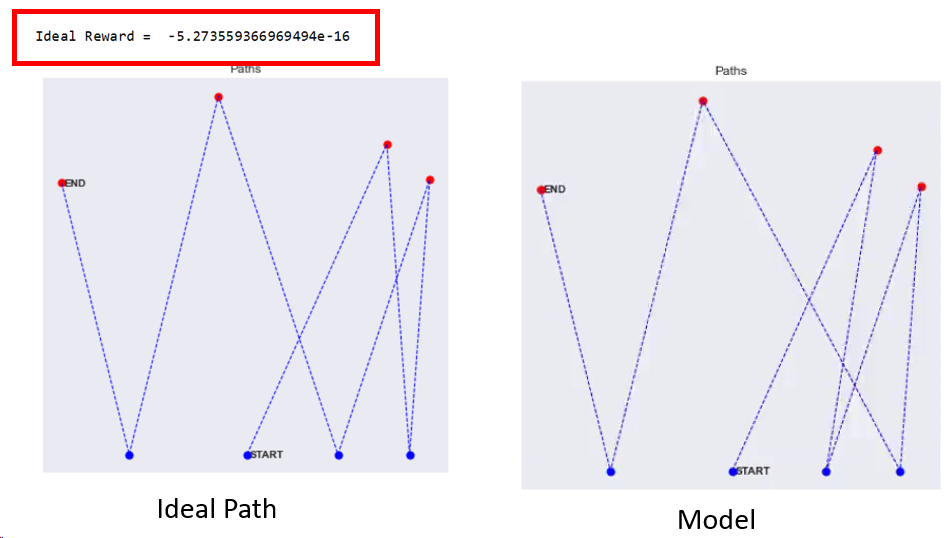
\includegraphics[width=0.7\textwidth]{8pt}
	\caption{~Optimal vs Model Path Comparison}
	\label{fig:8pt}
\end{figure}

\centering{
$Accuracy = \frac{\text{Number Of Iterations with Optimal Results}}{\text{Number Of Testing Iterations}}$}

\begin{figure}[h]
	\centering
	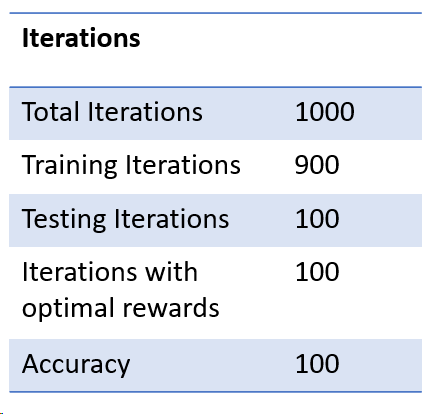
\includegraphics[width=0.3\linewidth]{8table}
	\caption{~Data Table}
	\label{fig:8table}
\end{figure}

\begin{figure}[h]
	\centering
	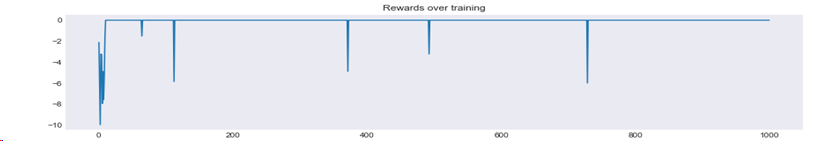
\includegraphics[width=0.9\linewidth]{8reward}
	\caption{~Reward Function Graph}
	\label{fig:8reward}
\end{figure}



\pagebreak
\justifying
\textbf{26 Point Incident Configuration}

\begin{figure}[h]
	\centering
	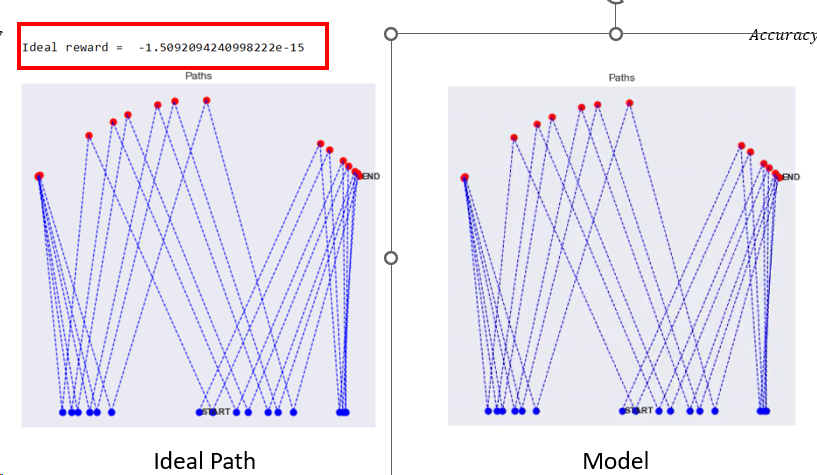
\includegraphics[width=0.7\textwidth]{26pt}
	\caption{~Optimal vs Model Path Comparison}
	\label{fig:8pt}
\end{figure}

\begin{figure}[h]
	\centering
	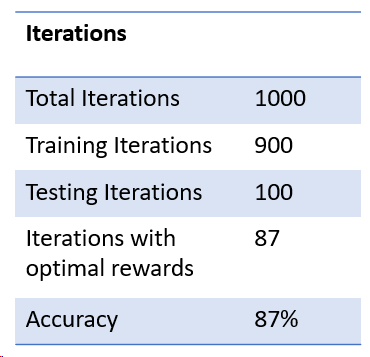
\includegraphics[width=0.3\textwidth]{26table}
	\caption{~Data Table}
	\label{fig:8table}
\end{figure}
\centering
$Accuracy = \frac{\text{Number Of Iterations with Optimal Results}}{\text{Number Of Testing Iterations}}$
\begin{figure}[h]
	\centering
	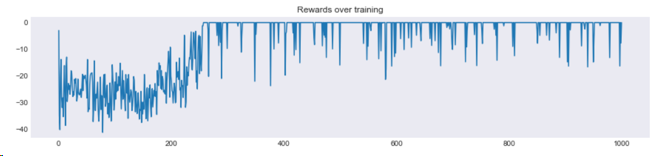
\includegraphics[width=0.6\textwidth]{26rewardfunc}
	\caption{~Reward Function Graph}
	\label{fig:reward}
\end{figure}

\newpage

\begin{figure}
	\centering
	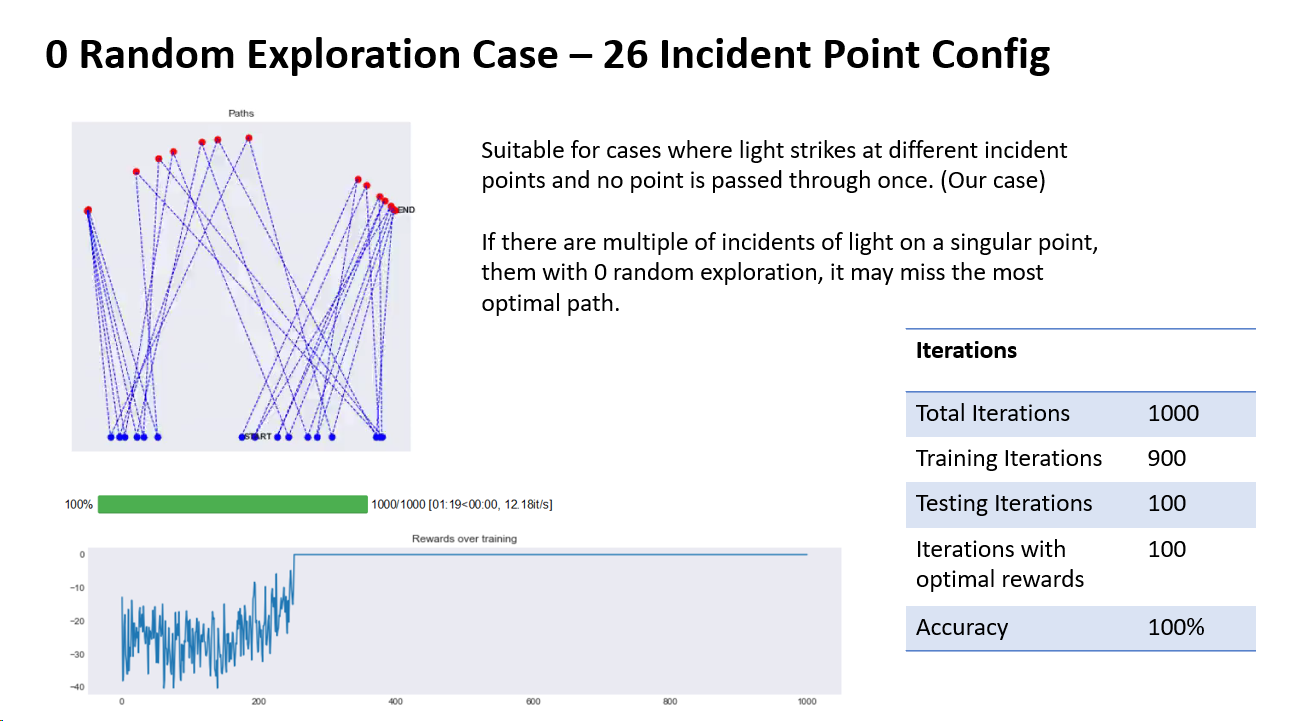
\includegraphics[width=1\linewidth]{26pt1}
	\caption{~Greedy Exploration}
	\label{fig:26pt1}
\end{figure}
\subsection{Limitations}
\justifying
The current simulations do not consider noise in the input point coordinates, where slight variations in the x-coordinates of some points may occur. Investigating such cases would provide valuable insights into how the simulations respond to these changes and what implications they hold for the results obtained.

Furthermore, the existing implementation is not specifically optimized for back-tracing of the light ray. In scenarios where multiple sources of light pass through the same points, the simulations might encounter loops and get stuck in back-and-forth iterations between these points. This limitation suggests that the current approach may need further refinement to handle such situations more effectively and produce more accurate outcomes.
\newpage
\section{Conclusion}
\justifying

In conclusion, this project aimed to explore the behavior of light reflections when encountering an unknown reflective curve in a two-dimensional Cartesian plane. We investigated three distinct approaches to gain insights into the nature of these reflective curves.

The first approach, based on caustics and orthotomics, involved constructing orthotomics and caustic points of the curve with respect to our light sources. Although this approach provided valuable information about the reflective surface, we faced challenges in establishing a direct mapping between caustics and orthotomics with the curve, especially with discrete coordinate values.

The second approach, a brute force elimination method, involved running all permutations of possible successive reflections from the source of light to other incident points. Through this, we were able to filter out invalid paths based on the constraints of the plane mirror. However, the computational complexity of this approach limited its practicality for larger datasets.

The third approach, leveraging reinforcement learning, provided a more efficient and effective solution. The DeliveryQAgent class, customizing the QAgent class, allowed the agent to explore the delivery environment efficiently and find optimal paths. By remembering previously visited states and actions, the agent optimized its path and minimized exploration in already visited regions.

Through extensive simulations using the aforementioned approaches, we gained valuable insights into the behavior of light reflections on unknown reflective curves. While each approach had its strengths and limitations, the reinforcement learning method showed promise for future research in mapping the nature of reflective curves. It provided a balance between accuracy and computational efficiency, making it a suitable choice for practical applications.
 \begin{thebibliography}{}
	\bibitem{caustic}{Weisstein, Eric W. "Caustic." From MathWorld--A Wolfram Web Resource. https://mathworld.wolfram.com/Caustic.html }
	\bibitem{ortho}{Weisstein, Eric W. "Orthotomic." From MathWorld--A Wolfram Web Resource. https://mathworld.wolfram.com/Orthotomic.html }
	
	\bibitem{giblin}{Bruce, J. W., Giblin, P., 
		\& Gibson, C. G. (1981). On caustics of plane curves. American Mathematical Monthly, 88(9), 651. https://doi.org/10.2307/2320669}
	\bibitem{russian}{Dvoretskii, A. (2020). Caustics, Orthotomics, and Reflecting Curve with Source at an Infinity. In CEUR Workshop Proceedings.}
	
\end{thebibliography}
\end{document}